\chapter{Projeto 1: Implementação em Hardware PL}

Nesta primeira fase, o foco foi implementar a arquitetura apenas em PL. O caminho do sinal, desde a geração até à saída, foi desenvolvido e testado no Vivado. A Figura \ref{fig:relatorio_arquitetura_0} mostra a visão global da arquitetura implementada.

\begin{figure}[H]
    \centering
    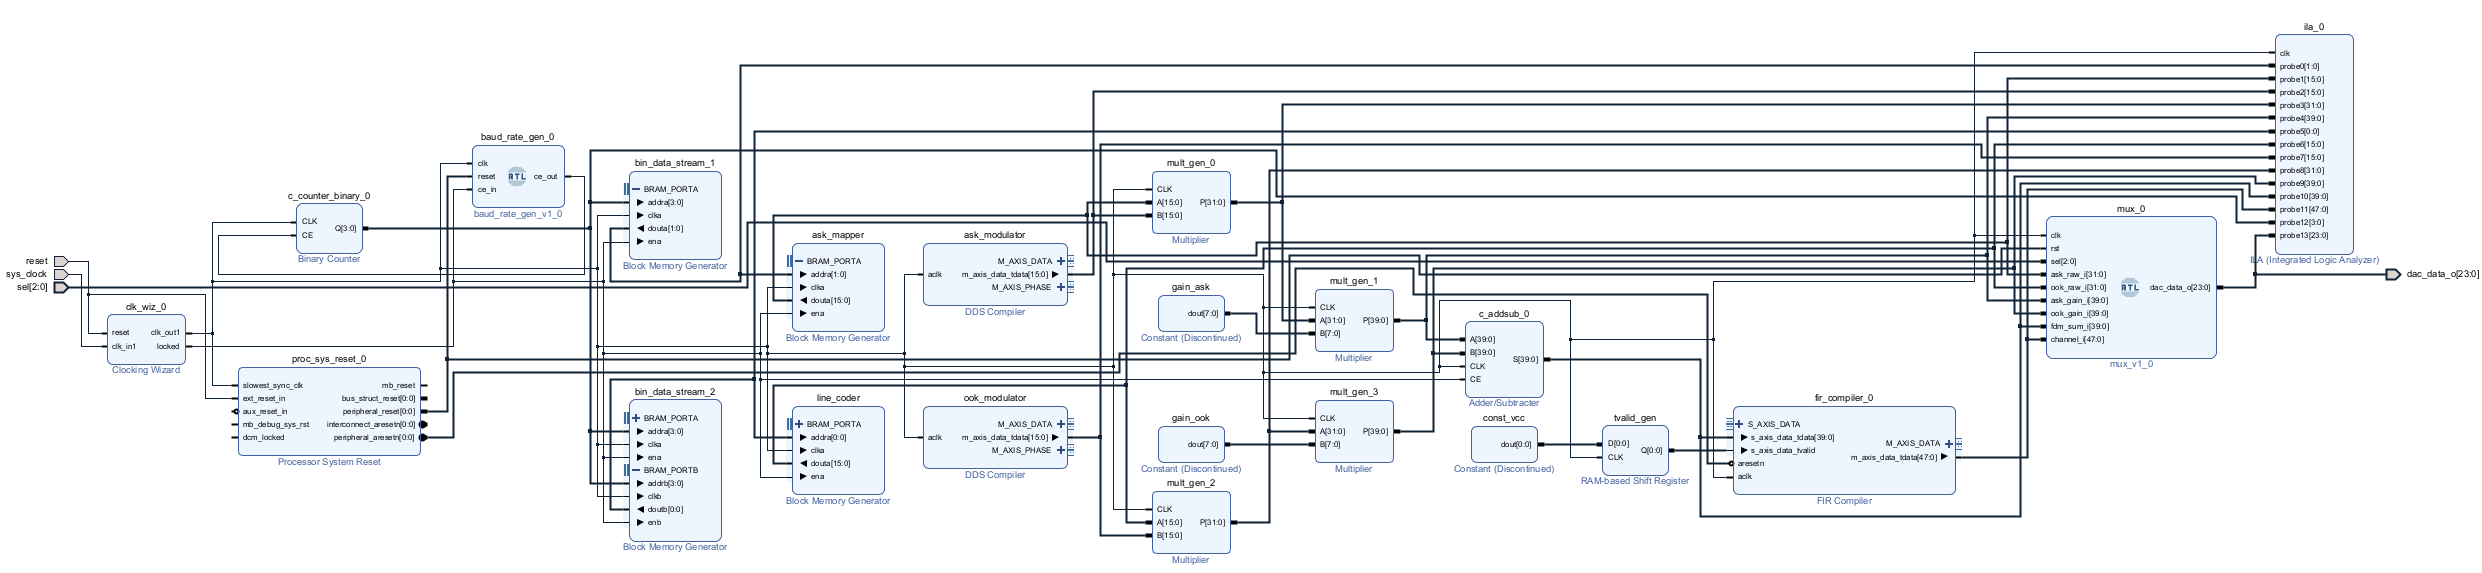
\includegraphics[width=\textwidth]{imgs/relatorio_arquitetura_0.png}
    \caption{Arquitetura global do sistema.}
    \label{fig:relatorio_arquitetura_0}
\end{figure}

\section{Geração de Dados e Moduladores}

A primeira parte do circuito gera os dados em banda base e mapeia-os em níveis de amplitude diferentes. Esta secção usa Block RAMs e compiladores DDS, como mostra a Figura \ref{fig:relatorio_arquitetura_1}.

\begin{figure}[H]
    \centering
    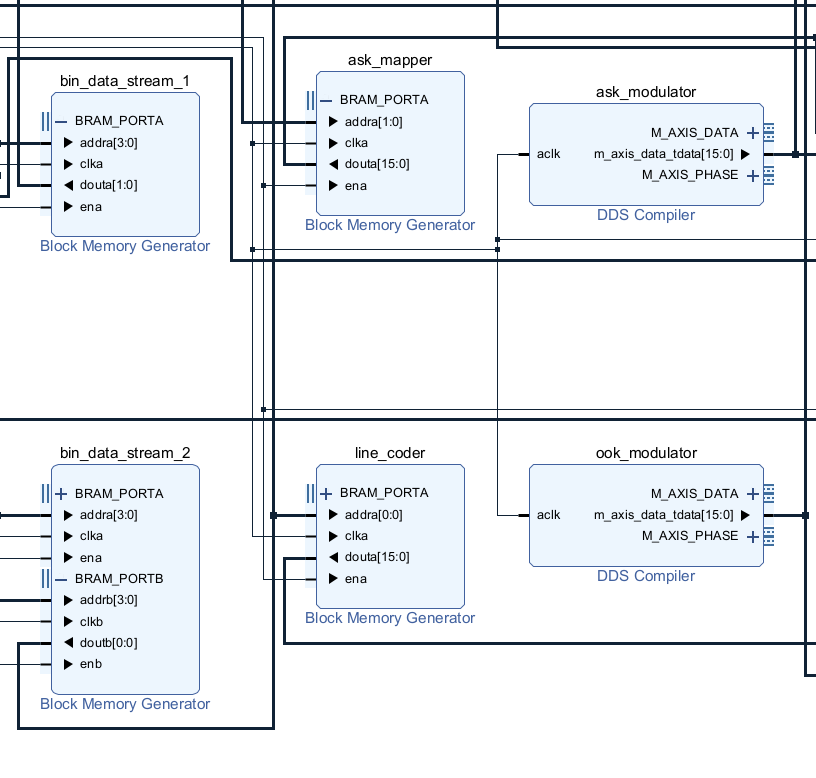
\includegraphics[width=\textwidth]{imgs/relatorio_arquitetura_1.png}
    \caption{Secção de Geração de Dados com BRAMs e Compiladores DDS.}
    \label{fig:relatorio_arquitetura_1}
\end{figure}

As Block RAMs funcionam como geradores pseudo aleatórios. O padrão cíclico de cada uma vem do ficheiro de inicialização usado para carregar a memória. Para o sinal ASK, a memória guarda valores em hexadecimal, com o vetor \texttt{0, 1, 2, 3, 0, 3, 1, 2, 1, 0, 3, 2, 3, 2, 1, 0}. Para o OOK, a via é binária, com a sequência \texttt{0, 1, 0, 1, 1, 0, 1, 0, 0, 1, 1, 0, 1, 0, 0, 1}.

Um bloco ASK Mapper converte esses valores nos 4 níveis de amplitude usados na modulação. O Line Coder converte o fluxo binário da via OOK. Neste Projeto 1, o nível do ASK vem só do ficheiro de inicialização e não se pode mudar em tempo real. O OOK está fixo ao código de linha NRZ.

A transmissão FDM precisa de portadoras sinusoidais para multiplicar o sinal em banda base. Estas são geradas por blocos Direct Digital Synthesizer (DDS): o ASK usa uma portadora a 1 MHz, e o OOK a 2 MHz.

\section{Ganhos, Multiplicadores e Somador}

Depois de geradas, as portadoras são multiplicadas pelos sinais das Block RAMs em blocos multiplicadores dedicados, o que completa a modulação em amplitude.

\begin{figure}[H]
    \centering
    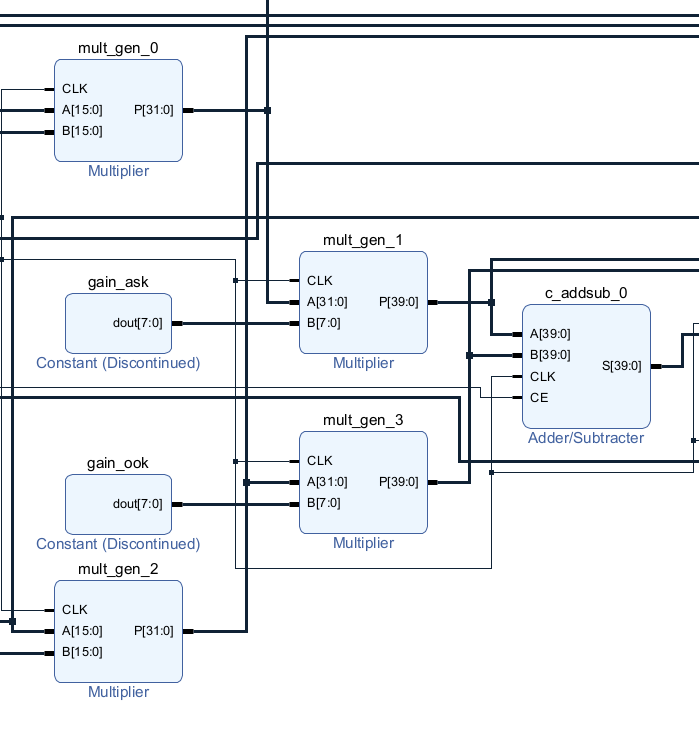
\includegraphics[width=\textwidth]{imgs/relatorio_arquitetura_2.png}
    \caption{Multiplicadores, blocos de ganho e somador FDM.}
    \label{fig:relatorio_arquitetura_2}
\end{figure}

O ganho de cada canal é controlado individualmente para equilibrar a potência na linha FDM, e este controlo acontece na mesma etapa da modulação. Como nesta fase o sistema é todo em lógica estática, os ganhos vêm de blocos de constantes e não podem ser alterados dinamicamente.

A junção FDM é feita num somador digital, no domínio linear. Como o relógio principal corre a 125 MHz, foi necessário ativar o pipeline interno do somador, para aliviar a lógica e cumprir os requisitos de timing.

\section{Emulação de Canal e Visualização}

Depois da transmissão, o sinal passa por um emulador de canal feito com um filtro FIR. Este IP corre em Single Rate, à taxa de amostragem de 125 MHz. O filtro serve para simular a atenuação de alta frequência que acontece num canal real, e foi desenhado com o algoritmo de Parks-McClellan. Tem 121 coeficientes, de 16 bits, com banda passante até 1.1 MHz e banda de rejeição a começar nos 1.9 MHz. Com isto, o canal ASK (1 MHz) passa sem distorção, enquanto o canal OOK (2 MHz) fica atenuado cerca de 32 dB, simulando as perdas do canal de transmissão.

\begin{figure}[H]
    \centering
    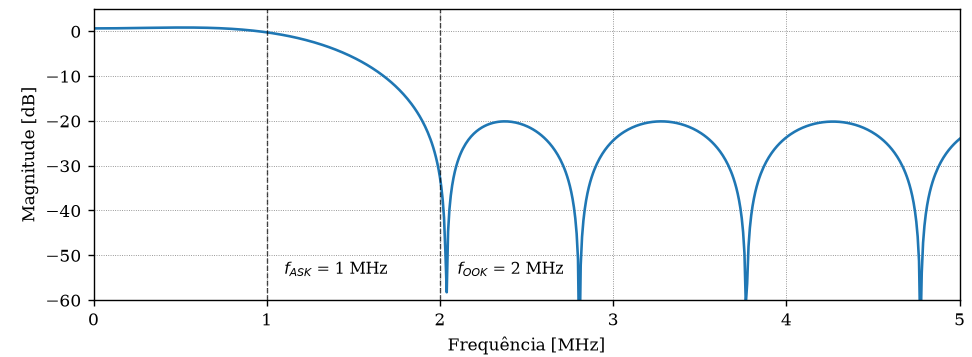
\includegraphics[width=0.8\textwidth]{imgs/fir_filter_response.png}
    \caption{Resposta em frequência e impulso do filtro FIR calculado.}
    \label{fig:fir_filter_response}
\end{figure}

\begin{figure}[H]
    \centering
    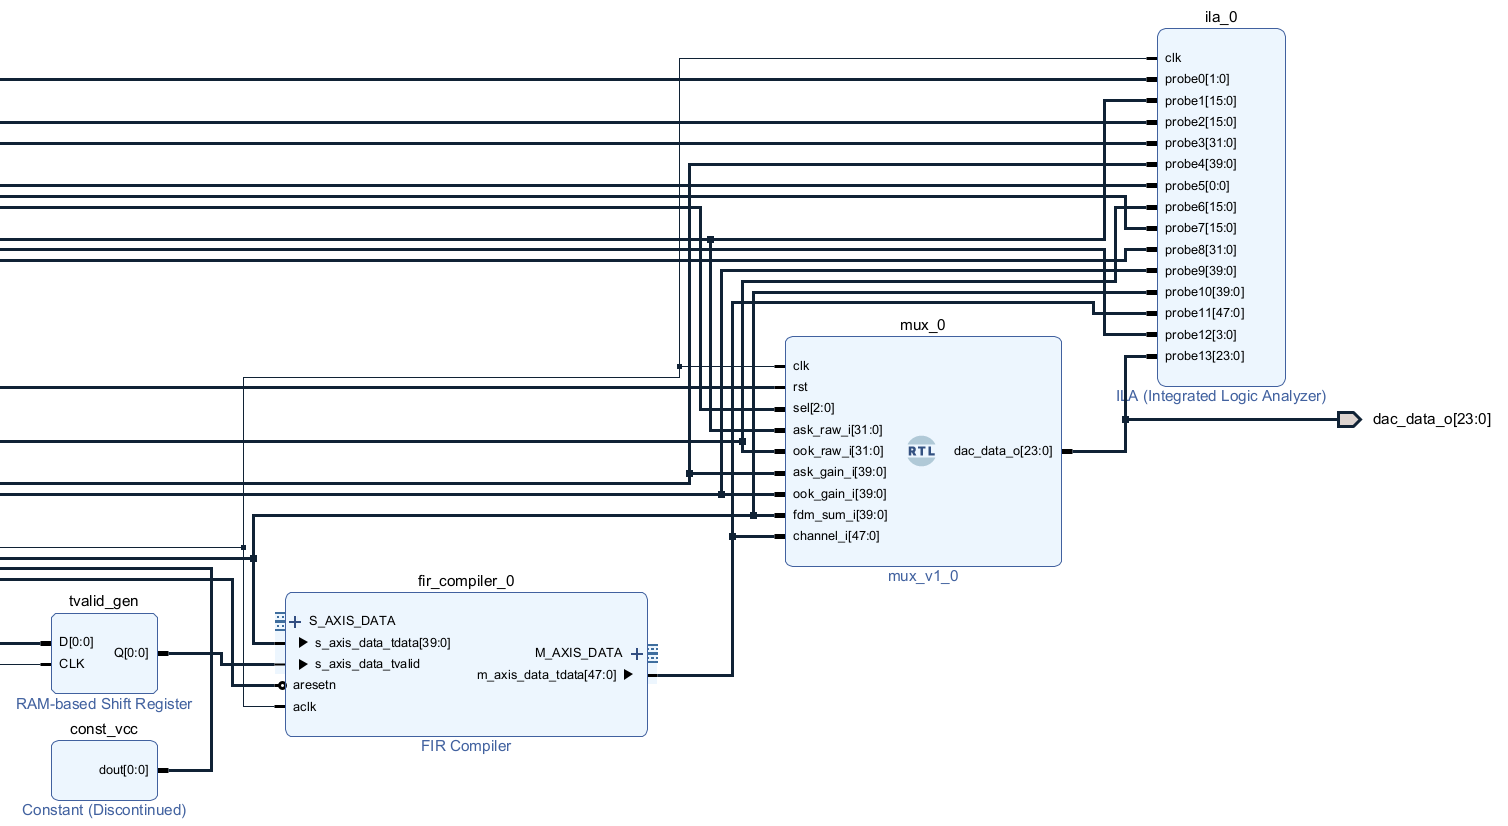
\includegraphics[width=\textwidth]{imgs/relatorio_arquitetura_3.png}
    \caption{Filtro FIR de emulação de canal, MUX de visualização e ILA.}
    \label{fig:relatorio_arquitetura_3}
\end{figure}

A multiplexagem de visualização foi materializada a partir de um MUX combinacional desenhado em VHDL para conduzir qualquer sinal requisitado ao barramento principal. O bloco DA2ref, que permitiria a averiguação prática via osciloscópio, estaria posicionado diretamente à frente do MUX caso estivesse implementado nesta fase. Atualmente o circuito apenas encaminha os dados e aciona a visualização em ferramentas de simulação. 

Como exemplos demonstrativos, onde a linha laranja é a saída do MUX, as linhas vermelha e azul são o sinal ASK e OOK com ganhos, respetivamente, apresentam-se os resultados através da simulação:

Quando acionada a segunda entrada do MUX através do bit de seleção 010, observa-se a representação intermédia do sinal ASK na Figura \ref{fig:relatorio_mux_2}.

\begin{figure}[H]
    \centering
    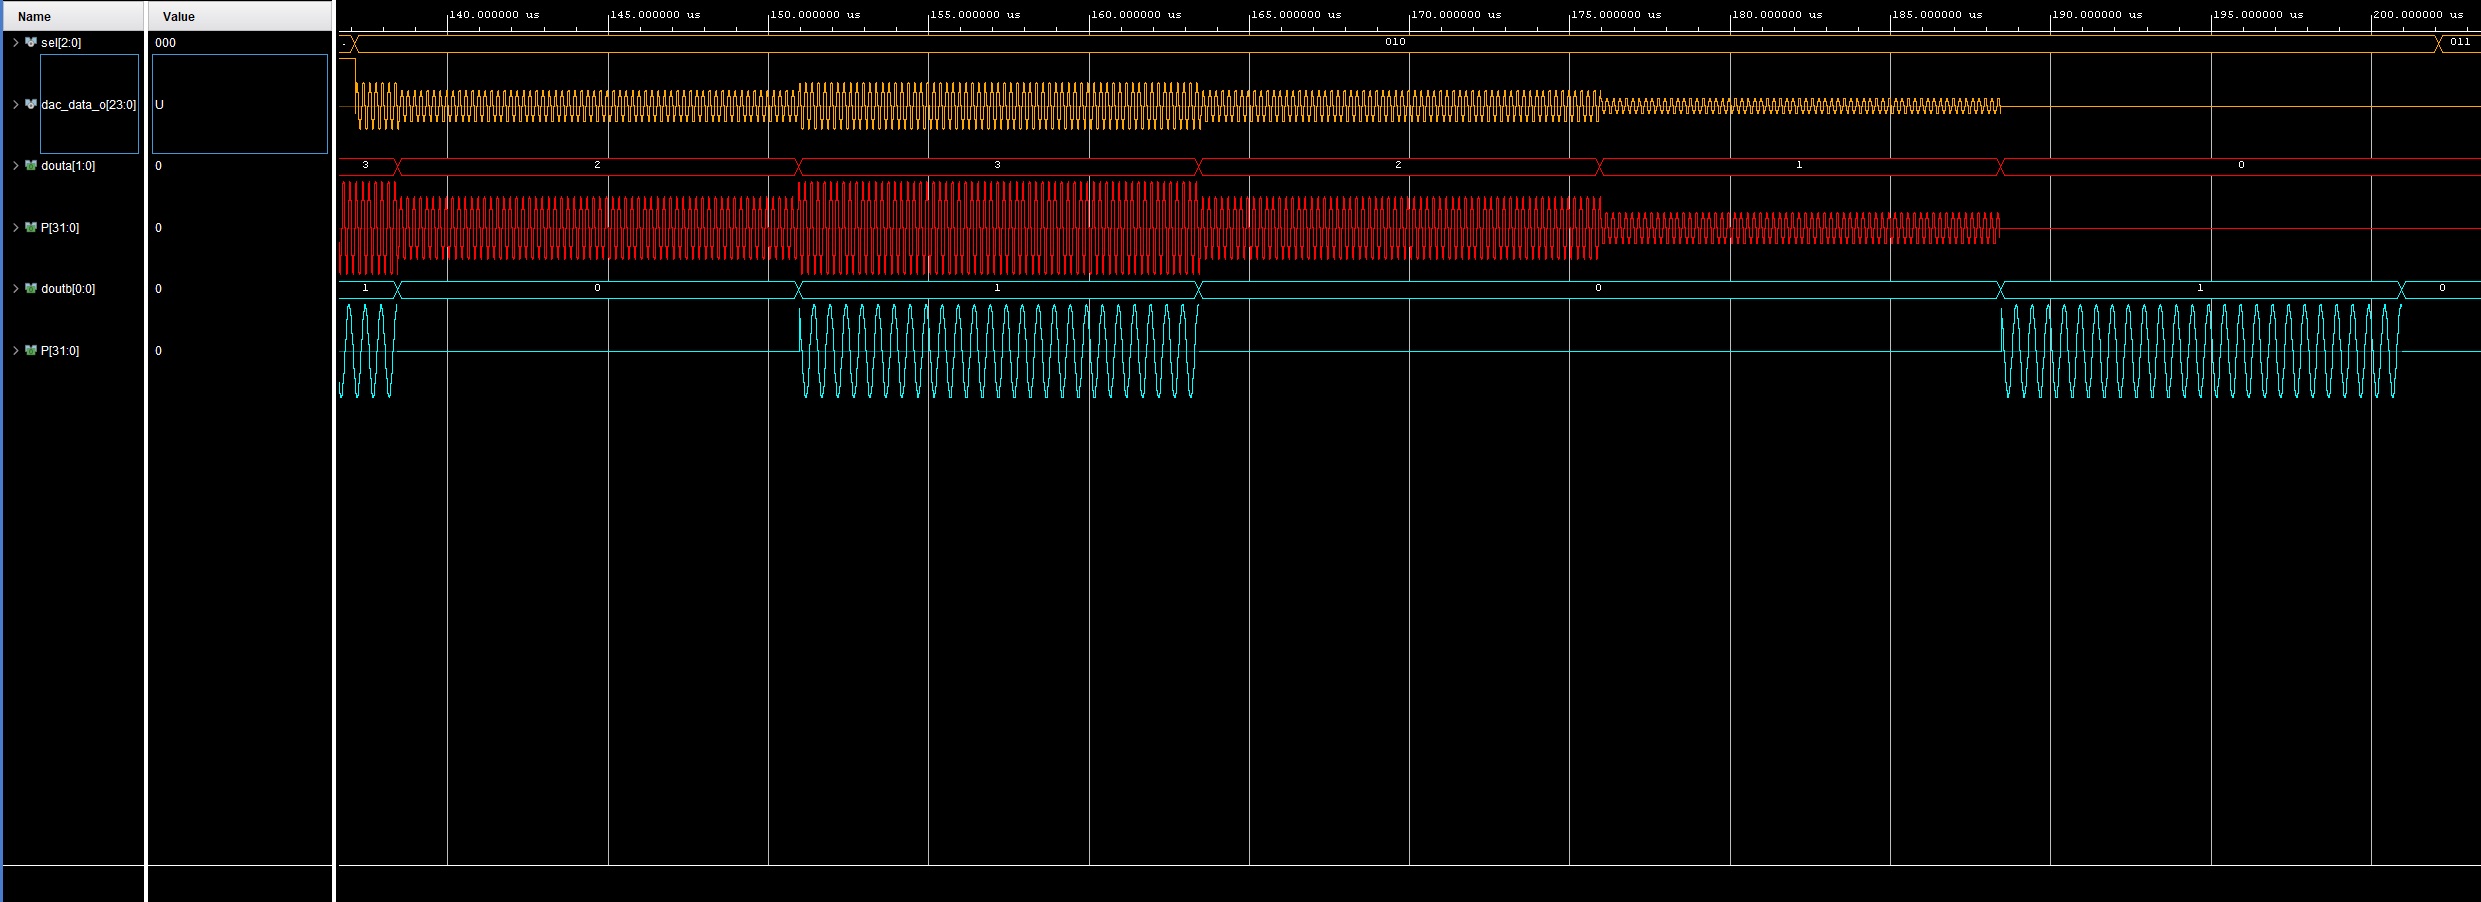
\includegraphics[width=\textwidth]{imgs/relatorio_mux_2.png}
    \caption{Visualização do estado lógico quanda seleção é 010.}
    \label{fig:relatorio_mux_2}
\end{figure}

Ao transitar para a terceira entrada configurada com o bit 011, é possível verificar a via de sinal do modulador OOK, tal como se pode verificar na Figura \ref{fig:relatorio_mux_3}.

\begin{figure}[H]
    \centering
    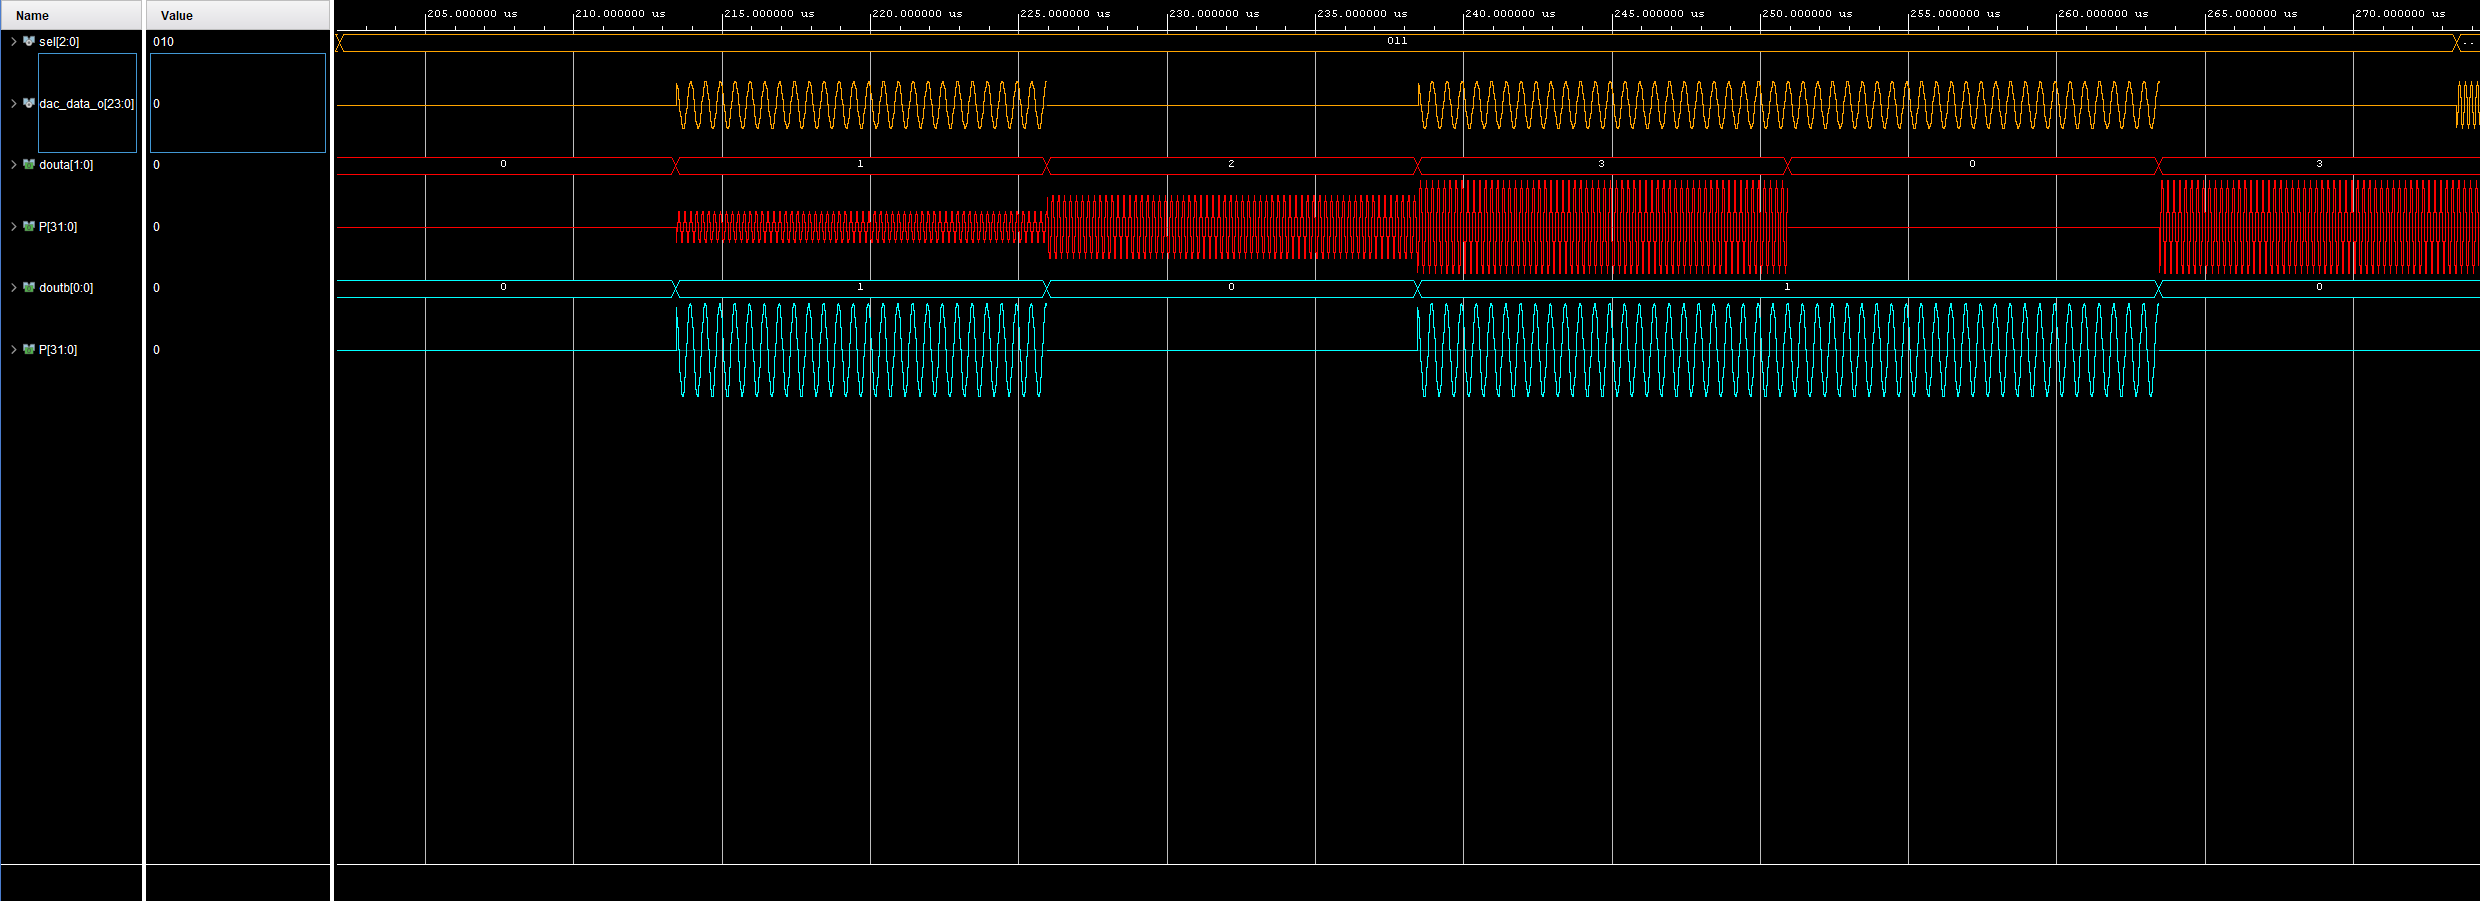
\includegraphics[width=\textwidth]{imgs/relatorio_mux_3.png}
    \caption{Visualização do estado lógico quanda seleção é 011.}
    \label{fig:relatorio_mux_3}
\end{figure}

Ao selecionar a quarta entrada (bit 100 na seleção), visualiza-se a via do sinal multiplexado conforme demonstra a Figura \ref{fig:relatorio_mux_4}.

\begin{figure}[H]
    \centering
    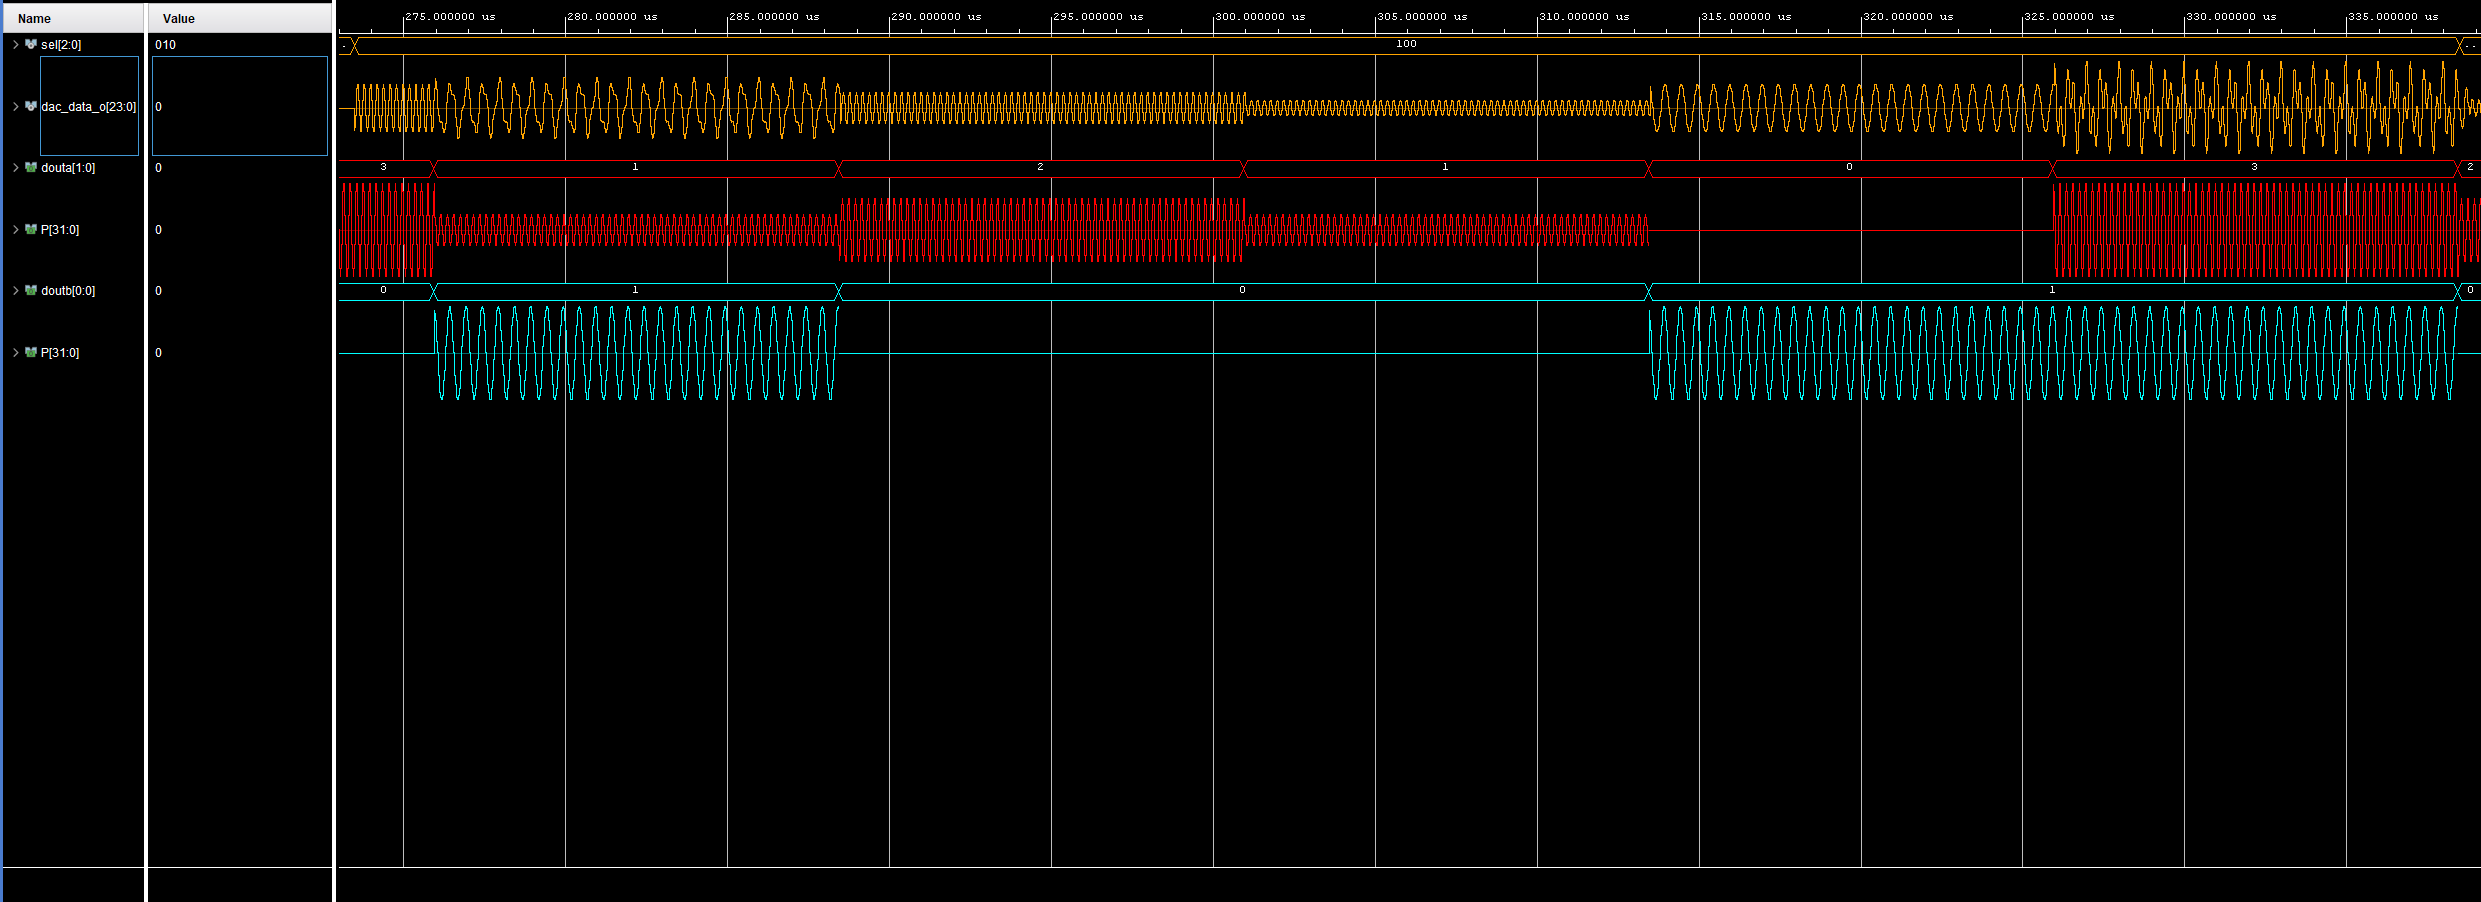
\includegraphics[width=\textwidth]{imgs/relatorio_mux_4.png}
    \caption{Visualização do estado lógico quanda seleção é 100.}
    \label{fig:relatorio_mux_4}
\end{figure}

Selecionando a última entrada com o bit 101, vemos a componente final da via. Aqui dá para ver o efeito direto do filtro FIR do emulador de canal: na primeira trama, o sinal OOK é zero, então a saída do FIR permanece a mesma que ASK. No momento que existam dados na linha OOK, o FIR atenua fortemente o sinal OOK, permanecendo apenas o sinal ASK. Na trama final, observa-se a ligeira atenuação do sinal OOK quando ASK é zero. Esta diferença confirma o comportamento seletivo do canal, como se vê na Figura \ref{fig:relatorio_mux_5}.

\begin{figure}[H]
    \centering
    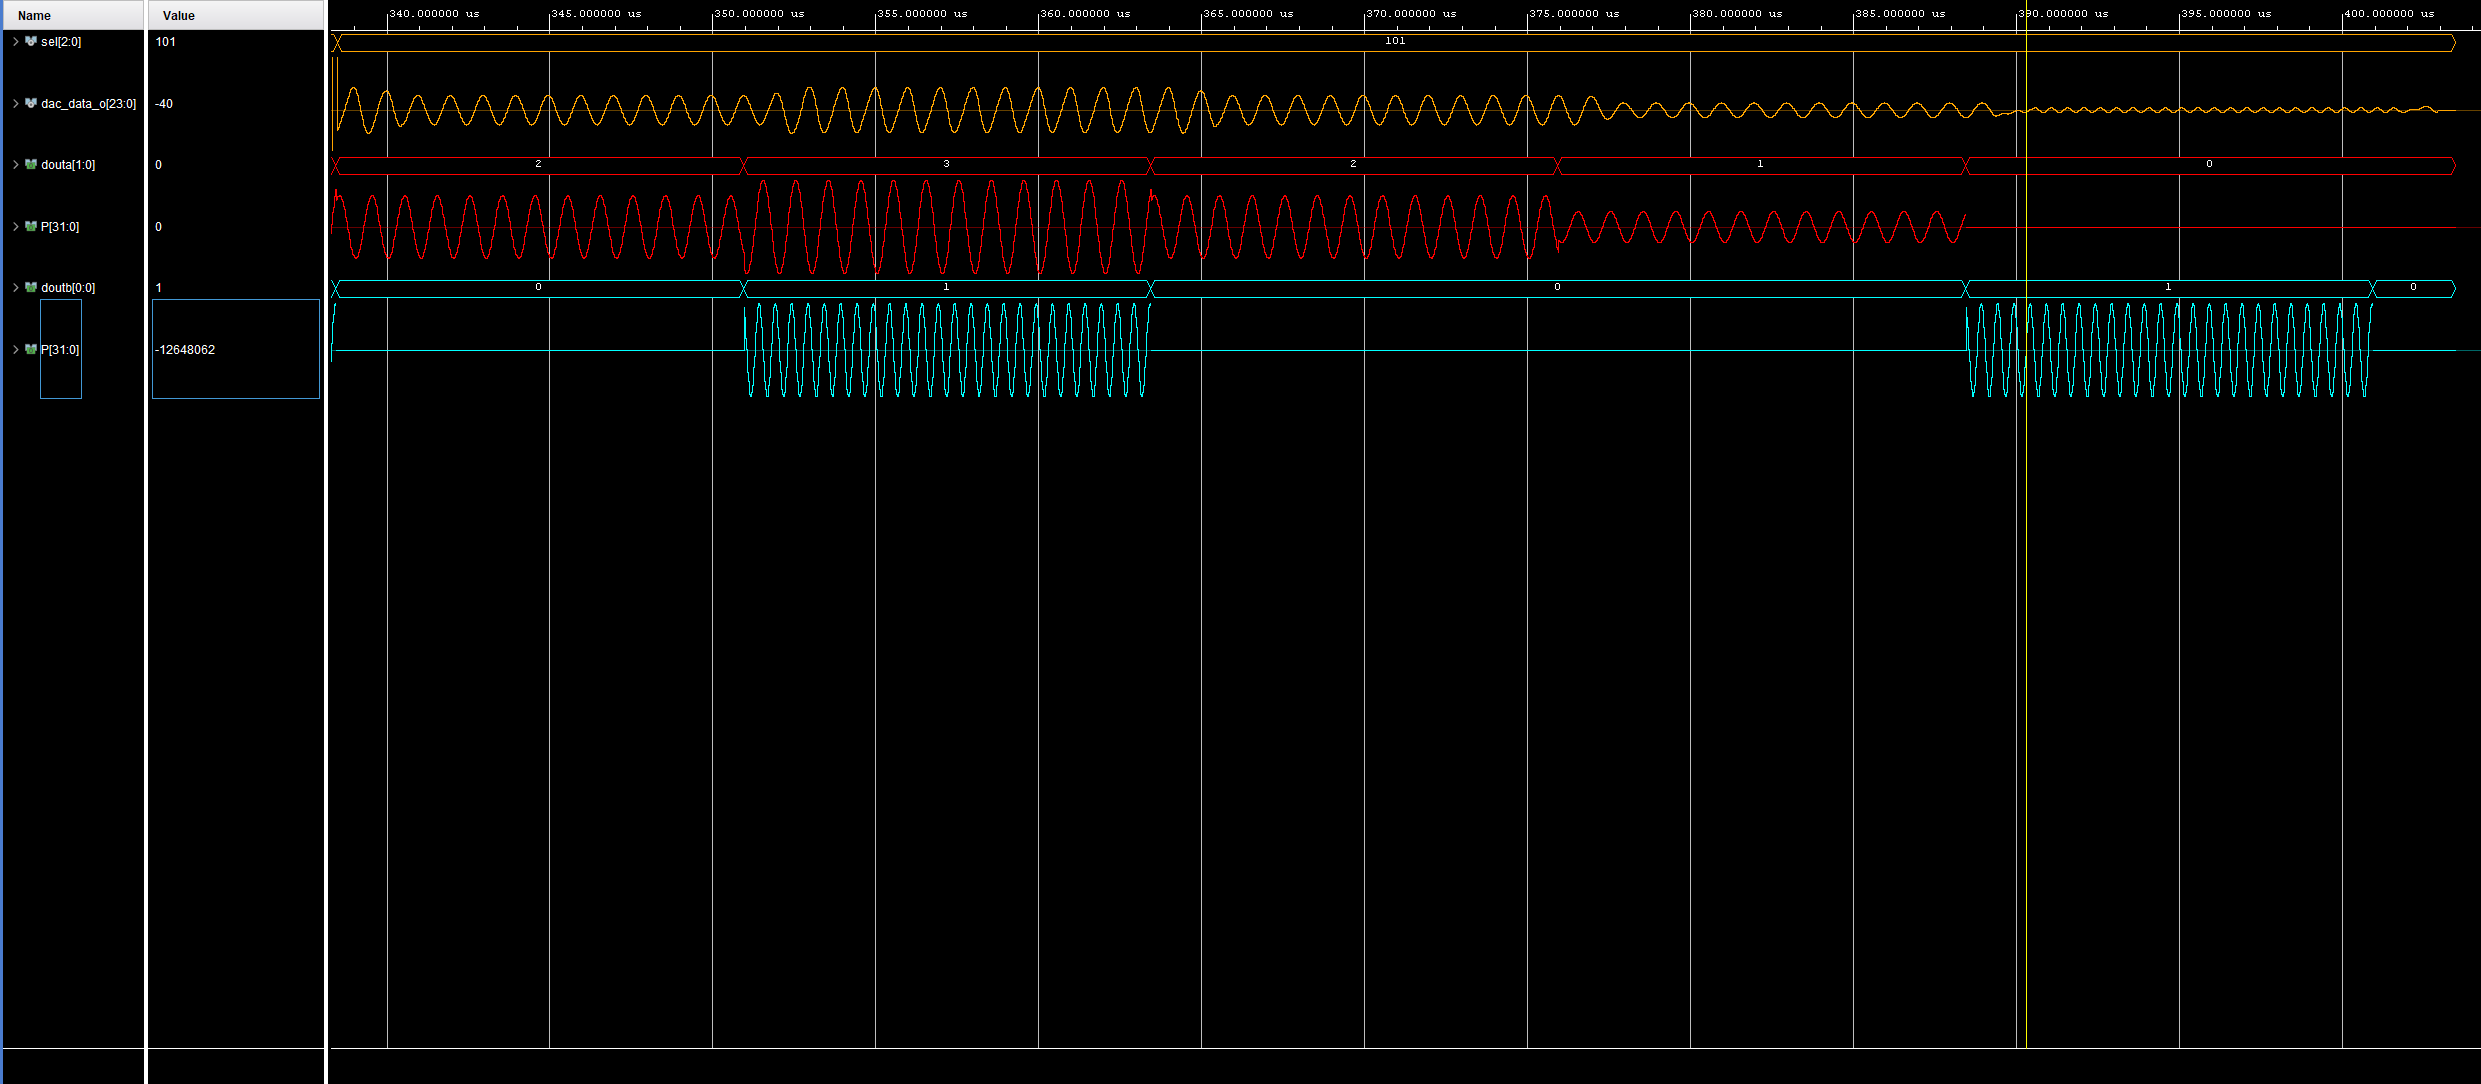
\includegraphics[width=\textwidth]{imgs/relatorio_mux_5.png}
    \caption{Visualização do estado lógico quanda seleção é 101.}
    \label{fig:relatorio_mux_5}
\end{figure}

Todos os sinais chegam também a um Integrated Logic Analyzer (ILA), o que permite no futuro fazer leituras diretamente na placa. Os processos e mapeamentos foram verificados em testbench, confirmando que as modulações implementadas funcionam como previsto.

\chapter{Projeto 2: Integração de Hardware e Software PS}

A segunda fase do projeto consiste na inserção do PS e na sua interligação com a PL. Este passo permite o controlo dos parâmetros de modulação e multiplexagem em tempo de execução.

\begin{figure}[H]
    \centering
    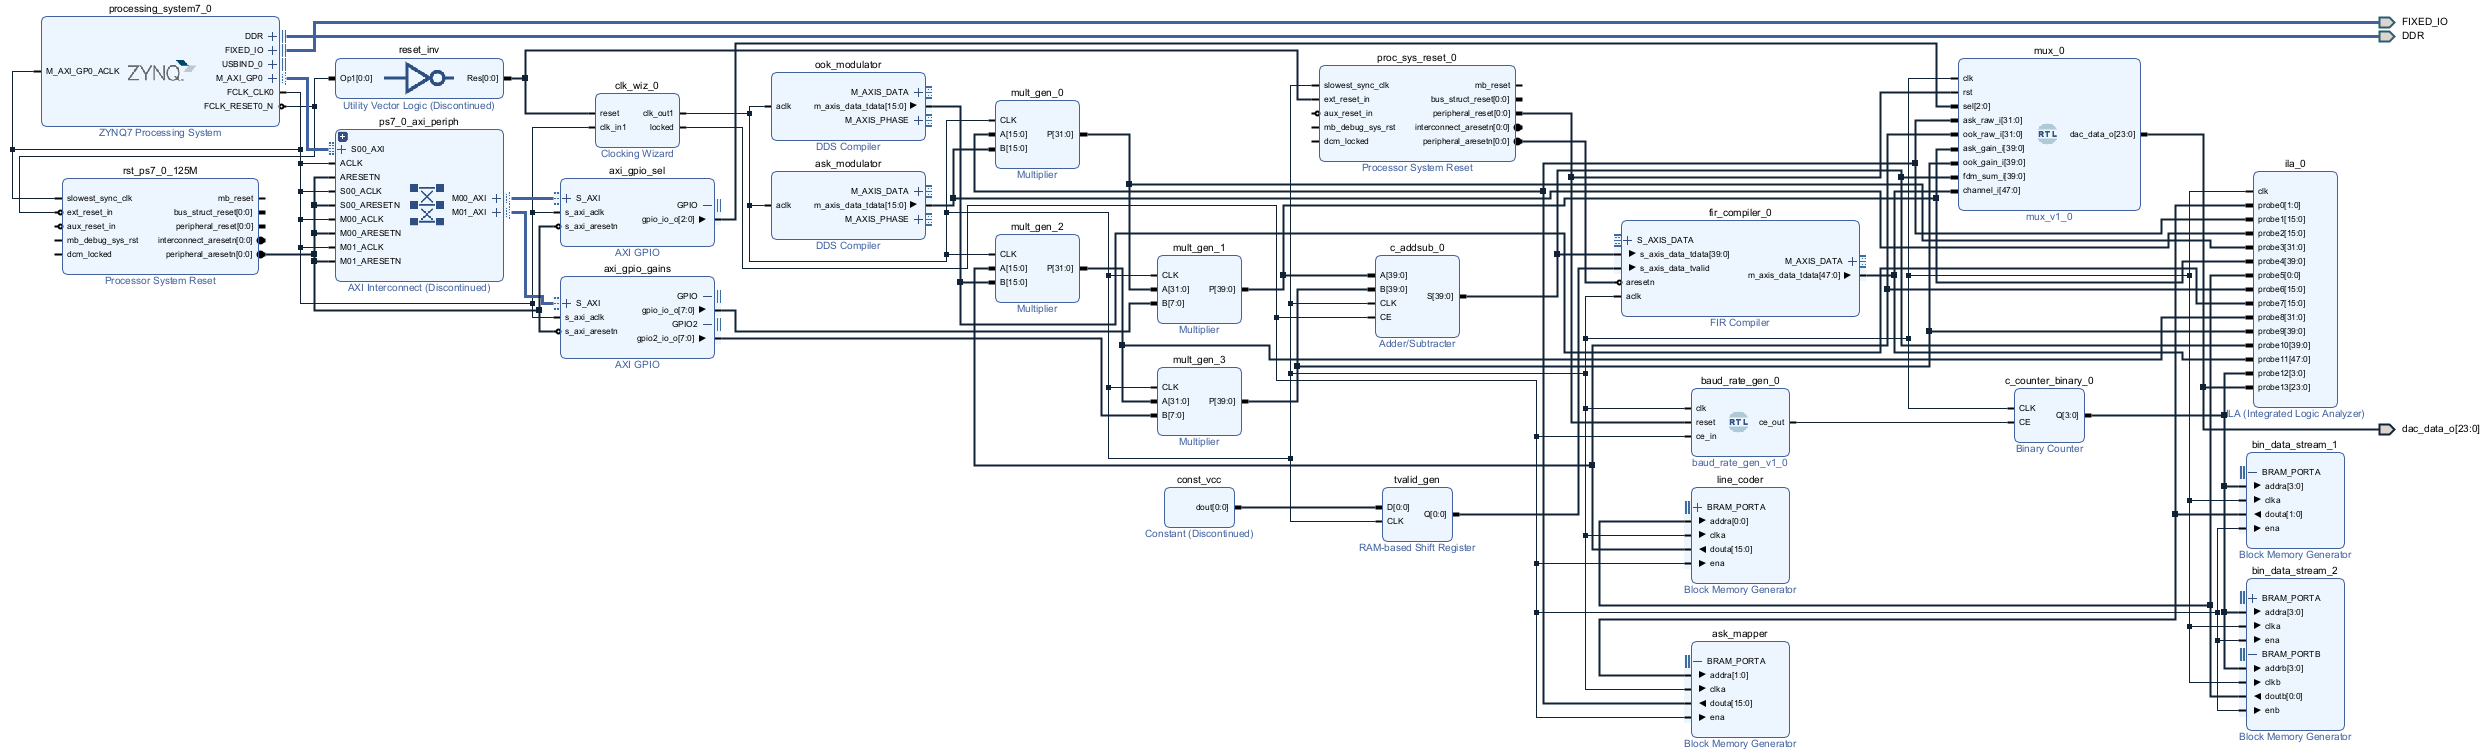
\includegraphics[width=\textwidth]{imgs/project_diagram_block_design.png}
    \caption{Diagrama de blocos do sistema.}
    \label{fig:project_diagram_block_design}
\end{figure}

\section{Sistema de Processamento e Barramento}

O processador atua como master na comunicação. O IP \texttt{processing\_system7\_0} fornece o sinal de relógio principal \texttt{FCLK\_CLK0}, de 125 MHz, e o sinal de reset de toda a parte logica. O PS tem como base um processador com arquitetura ARM e interage com memórias e periféricos, corre o sistema operativo Linux. A comunicação entre o processador e a FPGA é feita através de um IP AXI Interconnect, que traduz commandos de memória do PS em transações AXI4-Lite dirigidas aos periféricos slave.

\begin{figure}[H]
    \centering
    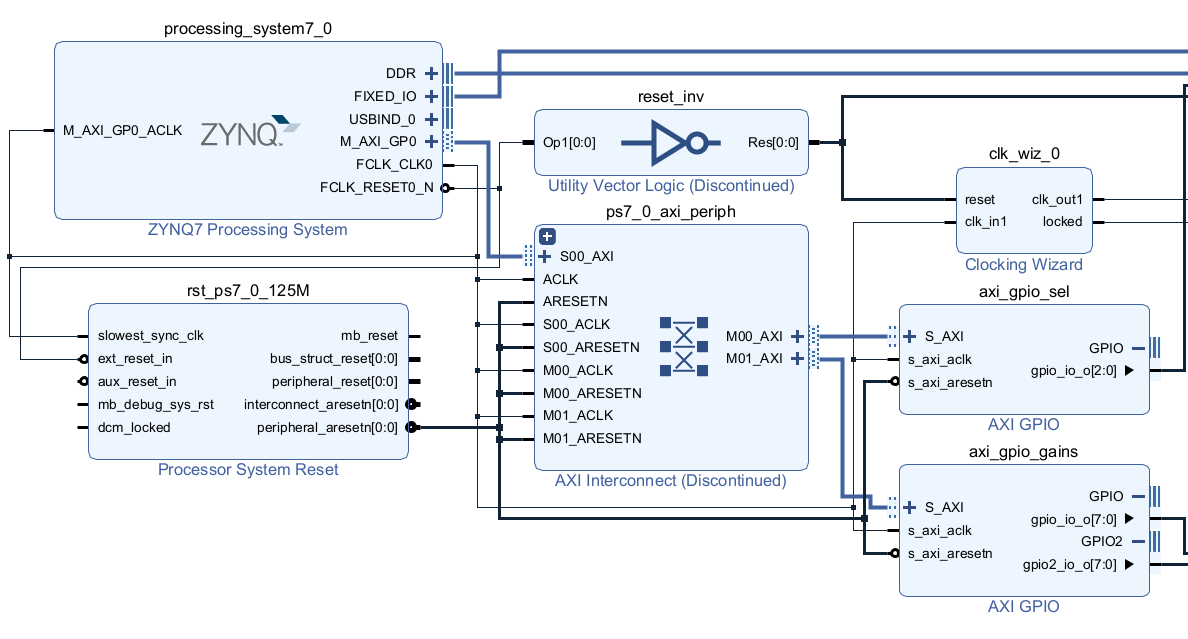
\includegraphics[width=\textwidth]{imgs/block_design_PS_axi_lite_axi_gpio.png}
    \caption{Detalhe do Zynq PS e interligação com os módulos AXI GPIO.}
    \label{fig:block_design_PS_axi_lite_axi_gpio}
\end{figure}

\section{Controladores de Periféricos}

Os blocos AXI GPIO funcionam como interface de modificação dos parâmetros dos caminhos de dados da modulação FDM, configurados como slaves AXI. O \texttt{axi\_gpio\_sel} tem um único canal, com largura de 3 bits, ligado à entrada de seleção \texttt{sel} do multiplexador. O \texttt{axi\_gpio\_gains} está configurado em dual channel, com os canais 1 e 2 a funcionar com largura de 8 bits: o canal 1 controla o ganho do ASK e o canal 2 o ganho do OOK.

O funcionamento interno dos GPIOs consiste em manter o valor recebido na porta AXI e na sua ligação aos pinos físicos ligados à lógica. A interação com o PS ocorre por Memory-Mapped I/O: cada escrita gera uma transação de 32 bits no barramento AXI, da qual apenas utiliza-mos o valor de 8 bits.

\begin{figure}[H]
    \centering
    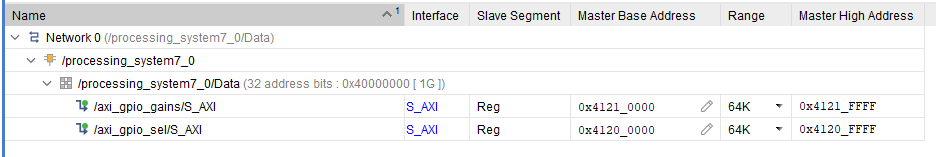
\includegraphics[width=\textwidth]{imgs/address_editor.png}
    \caption{Mapeamento de memória no Address Editor do Vivado.}
    \label{fig:address_editor}
\end{figure}

Os parâmetros configuráveis via GPIO são o ganho aplicado ao somador e o canal selecionado no multiplexador. Mudar estes valores muda o balanceamento de potência entre vias e o comportamento das saídas intermédias.

\section{Sincronização e Geração de Baud Rate}

O relógio do sistema vem do PS e tem frequência de 125 MHz. As portadoras usadas andam na ordem de 1 MHz e 2 MHz. Se a sequência em banda base for lida a 125 MHz, esta sobrepõe-se à portadora e o sinal modulado sai distorcido. Por isso foi criado o bloco \texttt{baud\_rate\_gen.vhd}, que faz a divisão do relógio.

Este módulo gera uma nova baud rate para as memórias BRAM. As entradas são o relógio do sistema e um reset síncrono, a saída é um impulso digital. Por dentro, tem um contador síncrono que conta ciclos de relógio, quando chega aos 1250 ciclos, o impulso de saída fica a 1 lógico. Este bloco não fala com o barramento do PS. Com este divisor, a baud rate do sistema FDM fica em 100 kHz.

\section{Interface de Software PYNQ}

O sistema é controlado a partir de uma aplicação Python na framework PYNQ. A aplicação carrega o bitstream \texttt{.bit} e o ficheiro com a descrição de hardware \texttt{.hwh}. A biblioteca \texttt{pynq.Overlay} serve para instanciar o overlay e aceder aos endereços dos módulos \texttt{axi\_gpio\_sel} e \texttt{axi\_gpio\_gains}.

\begin{figure}[H]
    \centering
    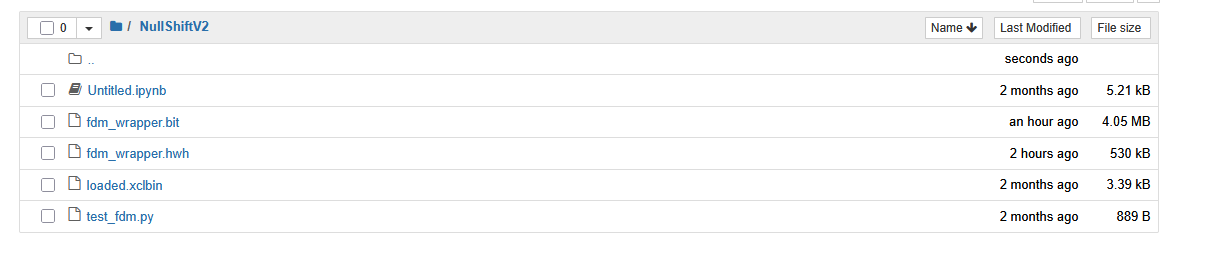
\includegraphics[width=\textwidth]{imgs/pynq_web_folder.png}
    \caption{Interface de gestão no ambiente Linux PYNQ.}
    \label{fig:pynq_web_folder}
\end{figure}

\begin{figure}[H]
    \centering
    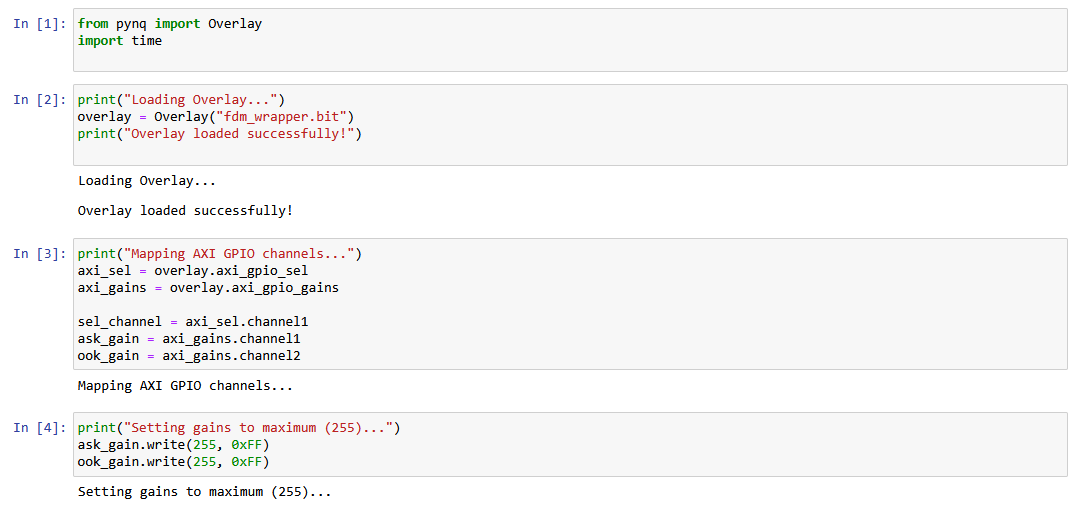
\includegraphics[width=\textwidth]{imgs/jupyter_1.png}
    \caption{Escrita de registos AXI Lite via Jupyter Notebook.}
    \label{fig:jupyter_1}
\end{figure}

Os scripts escrevem diretamente nas portas físicas através do barramento, preenchendo o resto do pacote com zeros de forma a agregar os 32 bits.

O controlo dinâmico do multiplexer e dos ganhos dos canais ASK e OOK foi testado no ambiente PYNQ, permitindo reconfigurar o sistema sem recompilar o hardware. No entanto, por instabilidades no ambiente de simulação e na interface do Vivado, não foi possível recolher e analisar as formas de onda em simultâneo com a variação destes parâmetros. Esta limitação foi agravada pela não implementação do bloco DAC na etapa final da cadeia de transmissão, o que impediu verificar os sinais com um osciloscópio físico.
